
\documentclass{jtetiproposalskripsi}

%-----------------------------------------------------------------
%Disini awal masukan untuk data proposal skripsi
%-----------------------------------------------------------------
\titleind{PENERAPAN APLIKASI DISTRIBUSI INFORMASI BERBASIS SMS GATEWAY PADA HIMPUNAN MAHASISWA ISLAM CABANG JEMBER}
\fullname{ELVRISKA AYU WIDIYANTI}

\idnum{1200631031}

\approvaldate{07 Januari 2015}

\degree{Sarjana Teknik Informatika}

\yearsubmit{2015}

\program{Manajemen Informatika}

\headprogram{Bagus Setya, S.T., M.T., Ph.D.}

\firstsupervisor{Victor Wahanggara, S.Kom}
\firstnip{12 09 739}

\secondsupervisor{Triawan Adi Cahyanto, M.Kom}
\secondnip{}


%-----------------------------------------------------------------
%Disini akhir masukan untuk data proposal skripsi
%-----------------------------------------------------------------

\begin{document}

\cover

\approvalpage

%-----------------------------------------------------------------
%Disini akhir masukan untuk muka skripsi
%-----------------------------------------------------------------

%-----------------------------------------------------------------
%Disini awal masukan Intisari
%-----------------------------------------------------------------
\begin{abstractind}
Perkembangan  teknologi informasi sekarang ini berkembang sangat pesat, salah satunya adalah perkembangan internet. Saat ini website merupakan salah satu media yang sering digunakan untuk mencari informasi untuk berbagai kepentingan yang bisa diperoleh dengan mudah dan cepat. Organisasi Himpunan Mahasiswa Islam merupakan suatu Organisasi yang bergerak di bidang agama, menyadari betapa pentingnya peranan Organisasi Himpunan Mahasiswa Islam dalam berupaya meningkatkan masyarakat yang beriman dan bertakwa. Pada daerah jember ini terdapat cabang yang menjadi tempat untuk suatu organisasi tersebut. Pada kennyataannya suatu organisasi yang telah berdiri pastinya ingin mendapatkan suatu anggota yang sangat aktif dan dapat bekerjasama secara adil dan bijaksana, dan tentunya cerdas dan cermat. 

Suatu organisasi pastinya berharap mempunyai sebuah sistem informasi yang lebih canggih yang sesuai dengan era globalisasi pada saat ini. Seiring dengan sepengetahuan saya, pada suatu organisasi HMI ini masih minimnya informasi yang diperoleh secara manual, tanpa mengarah kedalam dunia komputerisasi ataupun secara singkat dan cepat, seperti misalnya pada saat akan memberikan informasi kepada para anggota ketika akan mengadakan sebuah pertemuan untuk membahas suatu topik, pihak ketua atau perwakilan harus berusaha menghubungi no telepon satu per satu para anggota melalui via sms ataupun telf, dan itupun terkadang masih terdapat kesalahan atau kendala apabila tidak terdapat salah satu no anggota yang tercantum. 

Melihat situasi yang seperti ini maka sistem ini diharap menjadi sebuah solusi bagi suatu Organisasi HMI. Aplikasi Distribusi Informasi Berbasis SMS Gateway ini solusi yang tepat untuk organisasi HMI dalam memudahkan memberikan informasi secara cepat dan akurat. 
Tujuan dan manfaat dari penelitian ini adalah untuk membantu proses penyampaian informasi mengenai jadwal perkumpulan anggota HMI , dan berbagai macam kegiatan HMI di Kabupaten Jember.



\bigskip
\textbf{Kata kunci} : Aplikasi Distribusi Informasi Berbasis SMS Gateway di HMI Cabang Jember.
\end{abstractind}
%-----------------------------------------------------------------
%Disini akhir masukan Intisari
%-----------------------------------------------------------------

\tableofcontents
\addcontentsline{toc}{chapter}{DAFTAR ISI}
\selectlanguage{bahasa}\clearpage\pagenumbering{arabic}\setcounter{page}{1}

%-----------------------------------------------------------------
%Disini awal masukan untuk Bab
%-----------------------------------------------------------------
\chapter{PENDAHULUAN}

\section{Latar Belakang}
Semakin bertambah dan berkembangnya teknologi informasi di segala bidang, dapat menjadikan sebuah pemecahan masalah terhadap pengolahan data yang semakin kompleks dan majemuk. Terlebih lagi di era globalisasi saat ini dapat dikatakan hampir tidak ada batasan waktu dan tempat lagi untuk memperoleh berbagai macam informasi yang diinginkan. Terdapat berbagai cara untuk melakuan penyampaian informasi menggunakan teknologi informasi yang dapat digunakan, salah satu contohnya adalah sms (Short Message System). 

SMS adalah sebuah layanan yang dioperasikan dengan sebuah telepon genggam untuk mengirim atau menerima pesan-pesan pendek. SMS sangat berperan penting bagi suatu organisasi dalam melakukan suatu percakapan komunikasi terkait dengan organisasi. Dimana dalam suatu organisasi disetiap anggota pasti membutuhkan suatu komunikasidengan memanfaatkan sms sebagai mediatornya. Sms dirasa sebagai salah satu alternatif didalam melakukan pengiriman distribusi informasi dengan efektif karena informasi yang disampaikan berupa pesan teks yang mempunyai batas 160 karakter. Namun pada hakekatnya yang terjadi didalam suatu organisasi tersebut akan mengalami kendala jika dalam organisasi mempunyai banyak anggota sehingga dalam proses pengolahan penyampaian informasi terkadang mengalami suatu permasalahan misalkan tidak tersampaikanya pesan singkat dikarenakan terlalu banyak beban pesan yang akan disampaikan pada media handpone sehingga akan menimbulkan masalah baru yang dapat menyulitkan pengirim informasi dalam proses penyampaian pesan ke para anggota organisasi. Hal tersebut timbul dikarenakan adanya spesifikasi handphone yang minim sehingga proses pengolahan banyak memakan waktu.

Salah satu organisasi yang melakukan penerapan distribusi informasi melalui sms yaitu adalah HMI. HMI merupakan suatu jenis organisasi Kemahasiswaan, Perkaderan dan Perjuangan, yang bertujuan terbinanya insan akademis, pencipta, pengabdi yang bernafaskan Islam dan bertanggung jawab atas terwujudnya masyarakat adil makmur yang diridhoi Allah S.W.T. Menanggapi kendala-kendala komunikasi yang dilakukan melalui sms dengan maksud untuk mendistribusikan informasi juga terdapat banyak kendala yang lain. Kendala yang dialami dalam pendistribusian informasi melalui perangkat handphone  yaitu kendala terhadap penyebaran informasi yang tidak merata diakibatkan proses pengiriman terlalu banyak sehingga perangkat tidak mampu meampung beban proses, dan kesulitan  dalam proses pengolahan penyebaran informasi. Dari permasalahan tersebut maka diinginkan sebuah sistem yang dapat menanggulanginya, yaitu dengan menggunakan perangkat lunak untuk pengiriman sistem distribusi informasi berbasis sms gateway yang diintregasikan menggunakan perangkat keras komputer atau disebut server. Sistem yang dibuat ini akan menyimpan data informasi pada server, yang mana pada server proses arus pengiriman informasi diharapkan lebih ringan dan mempercepat penyebaran distribusi informasi. SMS Gateway merupakan sebuah system aplikasi yang digunakan untuk mengirim dan atau menerima SMS, dan biasanya digunakan pada aplikasi bisnis, baik untuk kepentingan broadcast promosi, servis informasi terhadap pengguna, penyebaran content produk / jasa dan lain lain. Sehingga dengan adanya penerapan aplikasi distribusi informasi berbasis sms gateway tersebut diharapkan akan memberikan sebuah alternatif terkait dengan manajemen pengolahan data informasi dalam proses pendistribusian informasi yang lebih mudah, selain itu sistem aplikasi yang dibangun tidak hanya mengandung sistem satu arah melainkan dua arah dimana para anggota juga bisa melakukan pengiriman informasi terkait dengan organisasi.

Berdasarkan pemaparan di atas, maka disimpulkan rencana untuk membangun sebuah sistem yang terkait dengan judul “Penerapan Aplikasi Distribusi Informasi Berbasis SMS Gateway Pada Himpunan Mahasiswa Islam Cabang Jember”.



\section{Rumusan Masalah}
Berdasarkan penjelasan latar belakang yang telah diuraikan di atas terdapat beberapa rumusan masalah sebagai berikut :
\begin{itemize}

\item[1.]	Bagaimana merancang aplikasi distribusi informasi pada HMI berbasis SMS Gateway?
\item[2.]	Bagaimana membangun aplikasi distribusi informasi dapat terintegrasi dengan SMS Gateway?
\item[3.]	Bagaimana menganalisis proses penyampaian informasi ke anggota HMI?
\end{itemize}




\section{Batasan Masalah}
Pada penulisan Tugas Akhir ini penulis hanya mengkaji masalah proses pemberian informasi kegiatan keanggotaan HMI yang sesuai agenda dan proses mendapatkan timbal balik informasi dari para anggota dengan menggunakan bahasa pemrograman java dan database MySQL, sehingga diluar masalah di atas tidak termasuk dalam kajian penelitian ini.

\section{Tujuan}
Adapun tujuan dibangunnya aplikasi distribusi informasi berbasis sms gateway pada HMI Cabang Jember sebagai berikut :
\begin{itemize}

\item[1.]	Untuk  merancang sistem distribusi informasi berbasis sms gateway.
\item[2.]	Membangun aplikasi distribusi informasi pada organisasi HMI cabang jember
\end{itemize}



\section{Manfaat}
Adapun manfaatyang dapat digunakan dari pembuatan program aplikasi distribusi informasi berbasis sms gateway ini adalah sebagai berikut :
\begin{itemize}

\item[1.]	Dapat memproses data kegiatan pada HMI secara komputerisasi yang sesuai dengan agenda yang telah terstruktur.
\item[2.]	Dengan adanya pembuatan aplikasi distribusi informasi tersebut diharapkan dapat mempermudah pemberian informasi kepada para anggota sesuai dengan agenda yang telah terstruktur.
\end{itemize}


%-------------------------------------------------------------------------------
\chapter{TINJAUAN PUSTAKA}                

\section{Sejarah Himpunan Mahasiswa Islam (HMI)}
HMI adalah suatu organisasi mahasiswa yang didirikan di Yogyakarta pada tanggal 14 Rabiul Awal 1366 H bertepatan dengan tanggal 5 Februari 1947 M, atas prakarsa Lafran Pane beserta 14 orang mahasiswa Sekolah Tinggi Islam Universitas Islam Indonesia. Sebelum lahirnya HMI, terlebih dulu berdiri organisasi kemahasiswaan bernama Perserikatan Mahasiswa Yogyakarta pada tahun 1946. Dirasa Perserikatan Mahasiswa Yogyakarta tersebut tidak memperhatikan kepentingan para mahasiswa yang masih menjunjung tinggi nilai agama, maka mahasiswa islam mendirikan organisasi kemahasiswaan yang berdiri dan terpisah dari Perserikatan Mahasiswa Yogyakarta. Pada tahun 1946 suasana politik di Indonesia khususnya Yogyakarta  mengalami suatu Polarisasi antara pihak Pemerintah. Polarisasi ini membawa sebagian besar mahasiswa yang berada dalam Perserikatan Mahasiswa Yogyakarta berorientasi kepada Partai Sosialis, dengan situasi yang demikian para mahasiswa yang berideologi murni tetap bersatu menghadapi Belanda mencegah setidak-tidaknya mengurangi efek-efek dari Polarisasi politik. Berbagai hal yang mendorong beberapa orang mahasiswa untuk mendirikan organisasi baru, meski harus mengalami suatu hambatan yang dianggap belum tepat. 

Namun melihat dari berbagai kondisi yang ada dirasa cita-cita yang sudah lama diharapkan itu perlu diwujudkan karena bila membiarkan Perserikatan Mahasiswa Yogyakarta lebih lama didominasi oleh Partai Sosialis adalah hal yang tidak tepat. Penolakan sikap tersebut mendapat dukungan dari berbagai pihak, tidak hanya dari kalangan mahasiswa Islam, melainkan juga mahasiswa yang beragama Non-Islam yang masih menjunjung teguh ideologi keagamaan.HMI merupakan suatu jenis organisasi Kemahasiswaan, Perkaderan dan Perjuangan, yang bertujuan terbinanya insan akademis, pencipta, pengabdi yang bernafaskan Islam dan bertanggung jawab atas terwujudnya masyarakat adil makmur yang diridhoi Allah S.W.T. Yang mana dalam HMI ini sudah meluas keberbagai penjuru.

\newpage
\subsection{Struktur Organisasi}
\begin{figure}[ht!]
\centering
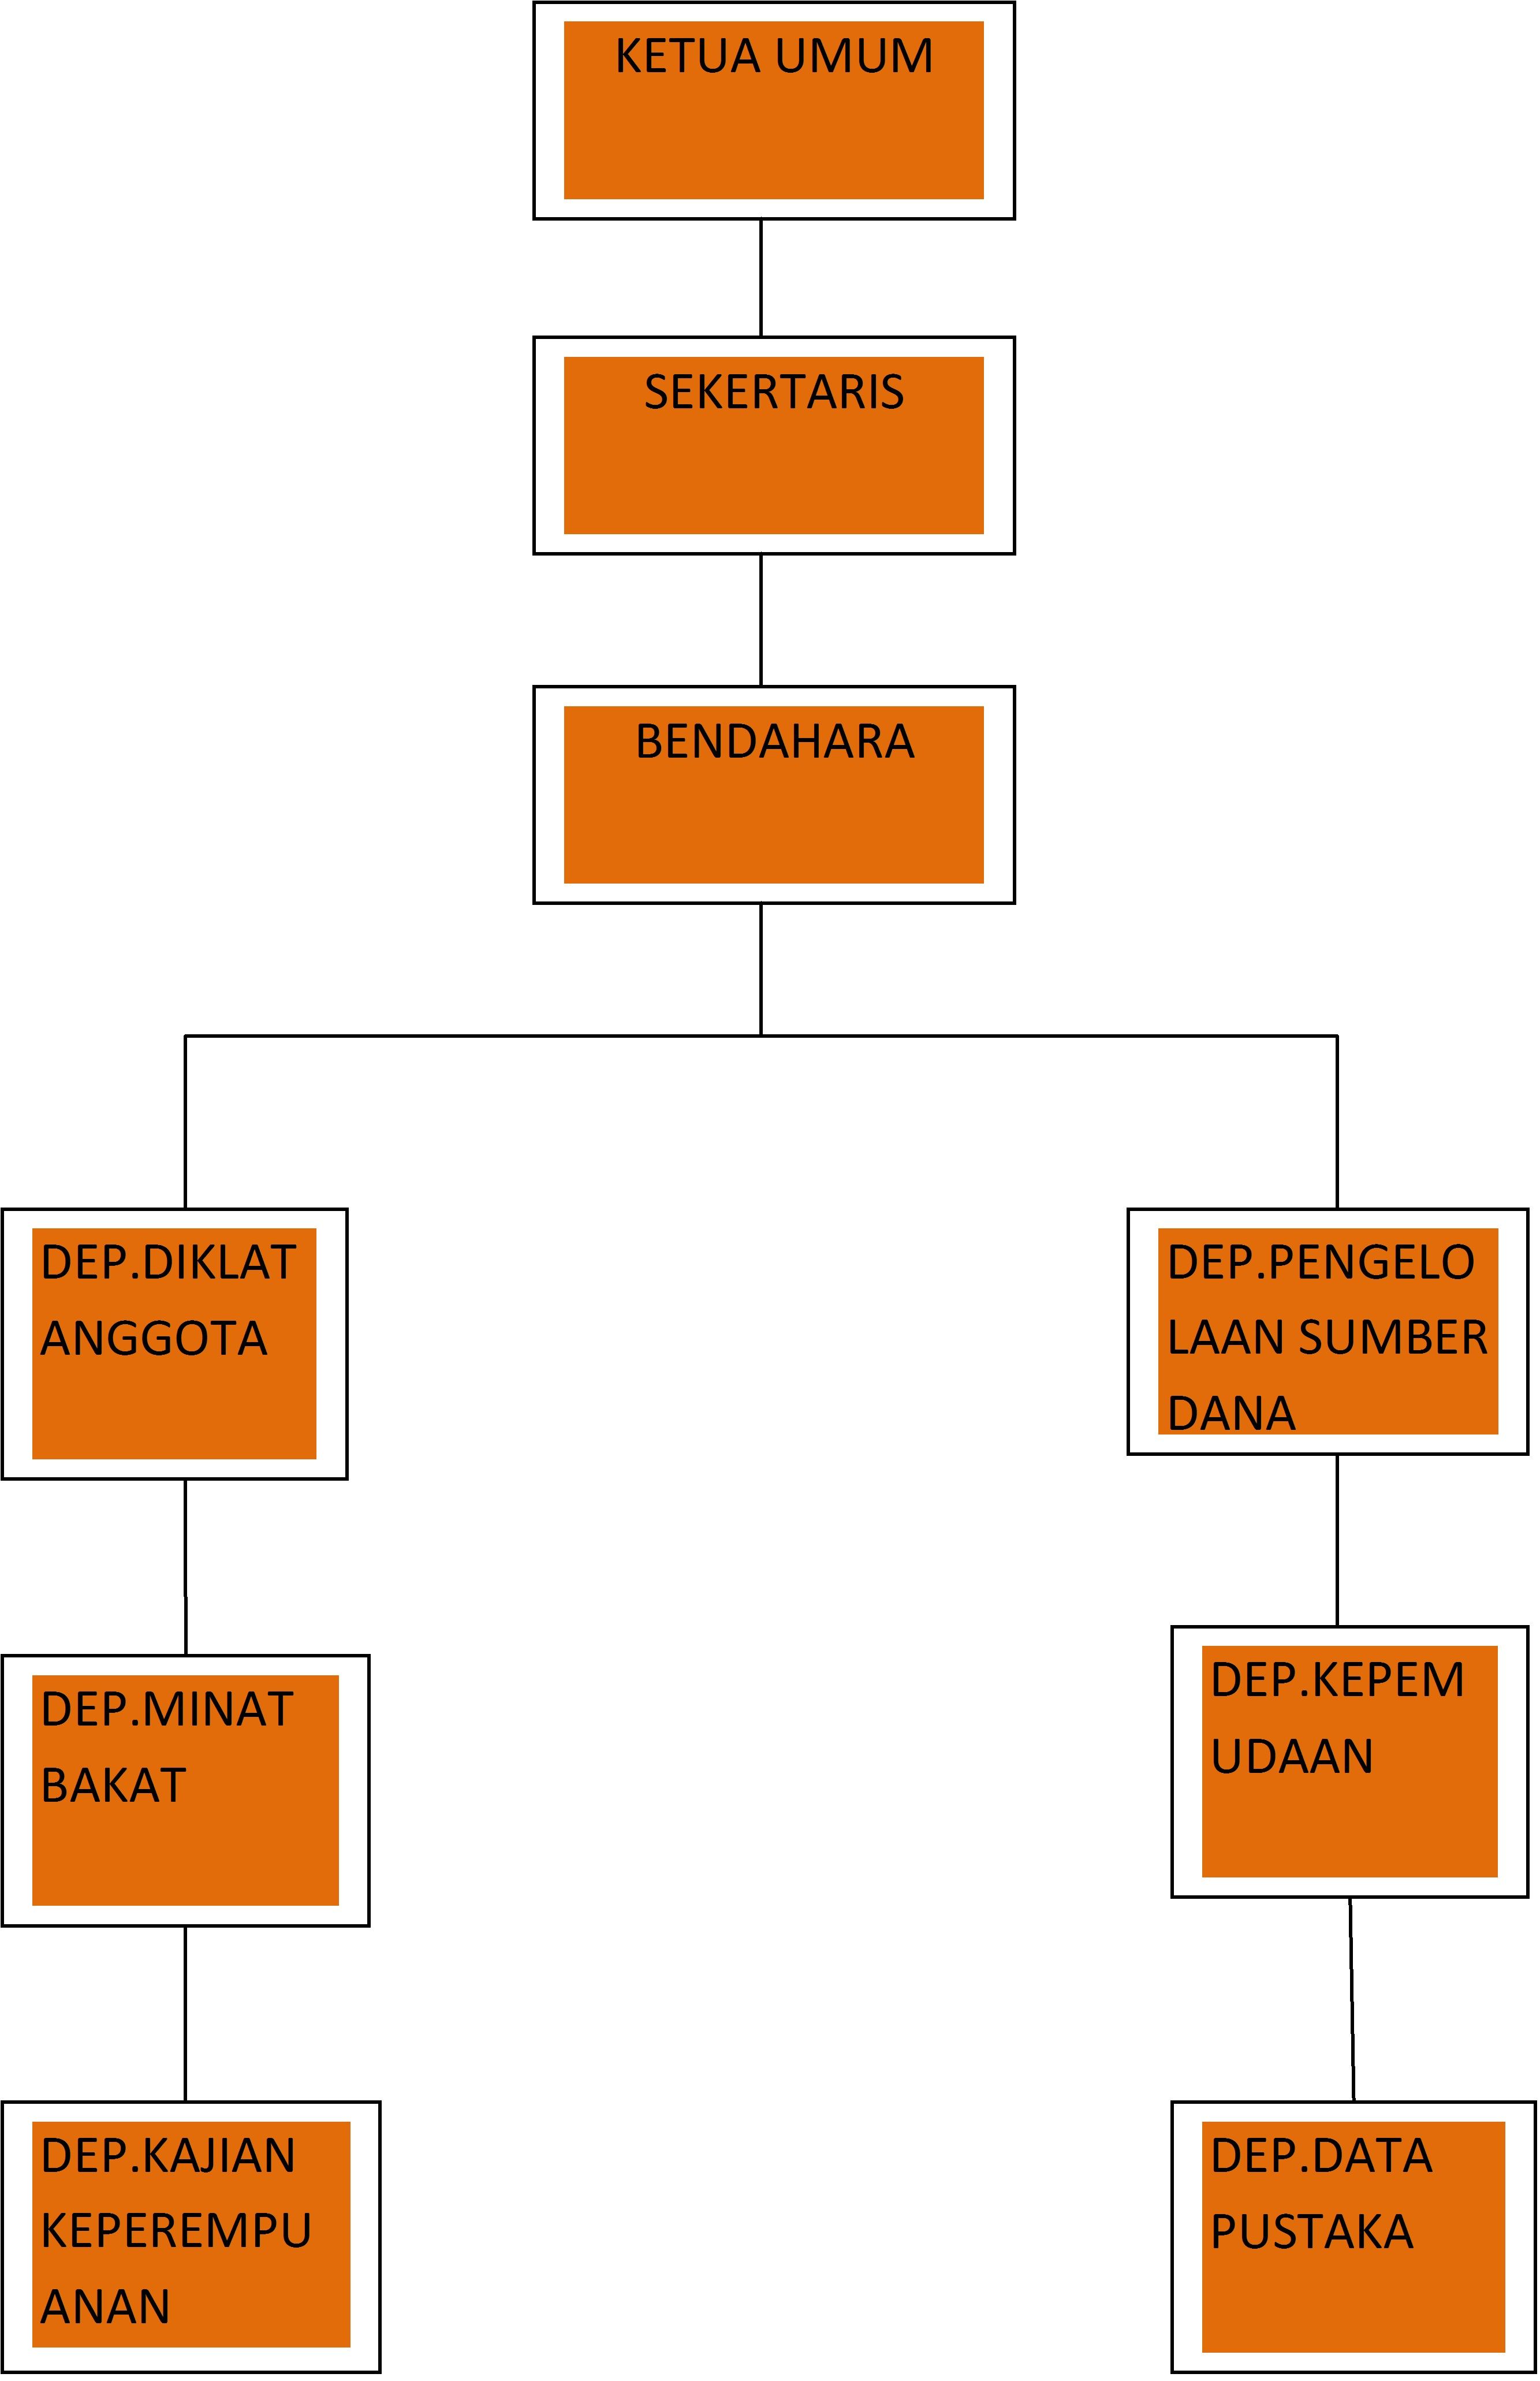
\includegraphics[width=0.8\textwidth]{gambar/Struktur}
\caption{\textit{Struktur Organisasi HMI}}
\label{wsn}
\end{figure}
\newpage

\section{Tinjauan Umum Sistem Infomasi}
\subsection{Sistem Informasi}
Menurut Tata Sutabri (2003: 3) sistem adalah kumpulan atau himpunan dari unsur, komponen atau variabel-variabel yang terorganisir, saling berinteraksi, saling tergantung satu sama lain dan terpadu untuk mencapai tujuan tertentu. Unsur dari sistem terdiri dari masukan (input), pengolahan (processing), dan keluaran (output). Pada dasarnya sesuatu dapat disebut sistem apabila memenuhi beberapa syarat, yaitu bila memiliki bagian (sub sistem) yang saling berinteraksi dengan maksud untuk mencapai suatu tujuan tertentu, dan harus memiliki unsur input sebagai penggerak atau pemberi tenaga di mana sistem itu dioperasikan, proses sebagai aktivitas yang mengubah input menjadi output, dan output sebagai hasil operasi. Jadi suatu sistem terdiri dari prosedur sebagai bagian-bagian yang saling berinterakasi dalam rangkaian unsur input, proses, dan output. 
	
Menurut Al-Bahra Bin Ladjamudin (2005:8) Informasi adalah hasil pengolahan data yang memberikan arti dan manfaat. Definisi informasi sebagai data yang telah diolah menjadi bentuk yang lebih berarti bagi penerimanya. Definisi informasi sebagai data yang telah diolah menjadi bentuk yang lebih berarti dan berguna bagi penerimanya untuk mengambil keputusan masa kini maupun yang akan datang.

Menurut Dr. Azhar Susanto, MBus, Ak (2004:55) Sistem Informasi adalah kumpulan dari sub-sub sistem baik phisik maupun non phisik yang saling berhubungan satu sama dan bekerja sama secara harmonis untuk mencapai satu tujuan yaitu mengolah data menjadi informasi yang berguna. sistem informasi merupakan gabungan dari komputer dan user yang mengelola perubahan data menjadi informasi serta menyimpan data dan informasi tersebut. (Jogiyanto. 2001)


\subsection{Distribusi Informasi}
Dalam kamus Bahasa Inggris – Indonesia, ”Distribution atau distribusi adalah pembagian, penyaluran”. I. Markus Willy. et.al(2005: 191). Distribusi sangat erat kaitannya dengan kegiatan perdagangan dan industri. Karena distribusi bagi sebagian pihak merupakan kegiatan utama yang mempengaruhi kegiatan lainnya secara keseluruhan. Banyak pihak yang berkaitan dengan kegiatan distribusi ini memperhatikan dengan teliti dan melakukan kegiatan ini dengan sebaik mungkin. Distribusi bagi sebagian pihak merupakan suatu hal yang penting, hal yang sangat menentukan dari keseluruhan kegiatan pihak tersebut. Sedangkan informasi adalah hasil pengolahan data yang memberikan arti dan manfaat. 

Maka definisi Distribusi informasi dalam suatu organisasi adalah cara-cara untuk memperoleh informasi dan berbagai informasi pada rekan kerja baik itu menggunakan metode-metode elektronik atau menggunakan arsip atau distribusi berkas secara manual.


\section{Tinjauan Singkat Perangkat Lunak}
\subsection{Software}
Nama lain dari Software adalah perangkat lunak. Karena disebut juga sebagai perangkat lunak, maka sifatnyapun berbeda dengan hardware atau perangkat keras, jika perangkat keras adalah komponen nyata yang dapat dilihat dan disentu holeh secara langsung manusia, maka software atau Perangkat lunak tidak dapat disentuh dan dilihat secara fisik, software memang tidak tampak secara fisik dan tidak berwujud  benda namun  bisa untuk dioperasikan. Software komputer adalah sekumpulan data elektronik yang disimpan dan diatur oleh komputer, data elektronik yang disimpan oleh komputer itu dapat berupa program atau intruksi yang akan menjalankan suatu perintah. Melalui software atau perangkat lunak inilah suatu komputer dapat menjalankan suatu perintah.


\subsection{Aplikasi}
Dalam suatu aplikasi bisa dikatakan sebagai software, akan tetapi suatu softare belum tentu bisa dikatakan sebagai aplikasi. Bila dimaknai secara istilah, aplikasi adalah suatu program yang siap untuk digunakan yang dibuat untuk melaksanakan suatu fungsi bagi pengguna jasa aplikasi serta penggunaan aplikasi lain yang dapat digunakan oleh suatu sasaran yang akan dituju. Menurut kamus komputer eksekutif, aplikasi mempunyai arti yaitu pemecah masalah yang menggunakan salah satu tehnik pemrosesan data aplikasi yang berpacu pada sebuah komputansi yang diinginkan atau diharapkan maupun pemrosesan dta yang diharapkan. Maka aplikasi merupakan proses atau prosedur aliran data dalam infrastruktur teknologi informasi yang dapat dimanfaatkan oleh para pengambil keputusan yang sesuai dengan jenjang dan kebutuhan (relevan).

\subsection{Java}
Java adalah bahasa pemrograman yang dapat dijalankan di berbagai komputer termasuk telepon genggam.  Bahasa ini banyak mengadopsi sintaksis yang terdapat pada C dan C++ namun dengan sintaksis model objek yang lebih sederhana serta dukungan rutin-rutin aras bawah yang minimal.  Aplikasi-aplikasi berbasis java umumnya dikompilasi ke dalam p-code (bytecode) dan dapat dijalankan pada berbagai Mesin Virtual Java (JVM). Java merupakan bahasa pemrograman yang bersifat umum/non-spesifik (general purpose), dan secara khusus didisain untuk memanfaatkan dependensi implementasi seminimal mungkin. Struktur dasar dari sintax java adalah seperti ini :

class test{

* @param args the command line arguments

public static void main(String[] args) {

// TODO code application logic here
}}

Berikut ini salah satu contoh syntax error, kita buka lagi program Hello.Java untuk dijadikan contoh perhatikan code dibawah ini :
\begin{figure}[ht!]
\centering
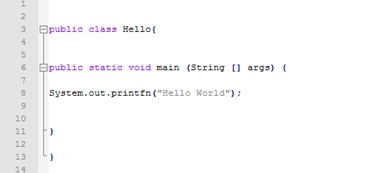
\includegraphics[width=0.6\textwidth]{gambar/koding}
\caption{\textit{Syntax Error}}
\label{wsn}
\end{figure}
\newpage

Contoh program sederhana dengan java :

// Outputs "Hello, world!" and then exits

publicclass HelloWorld {

publicstaticvoid main(String args[]){

System.out.println("Hello, world!");
	}
	}

Versi awal Java pada tahun 1996 sudah merupakan versi release sehingga dinamakan Java Versi 1.0. Java versi ini menyertakan banyak paket standar awal yang terus dikembangkan pada versi selanjutnya:
\begin{itemize}

\item[1.]	java.lang: Peruntukan kelas elemen-elemen dasar.
\item[2.]	java.io: Peruntukan kelas input dan output, termasuk penggunaan berkas.
\item[3.]	java.util: Peruntukan kelas pelengkap seperti kelas struktur data dan kelas kelas penanggalan.
\item[4.]	java.net: Peruntukan kelas TCP/IP, yang memungkinkan berkomunikasi dengan komputer lain menggunakan jaringan TCP/IP.
\item[5.]	java.awt: Kelas dasar untuk aplikasi antarmuka dengan pengguna (GUI)
\item[6.]	java.applet: Kelas dasar aplikasi antar muka untuk diterapkan pada penjelajah web.
\end{itemize}

Teknologi Java memiliki tiga komponen penting, yaitu:
\begin{itemize}

\item[1.]	Programming-language specification
\item[2.]	Application-programming interface
\item[3.]	Virtual-machine specification
\end{itemize}

\section{SMS Gateway}
SMS (Short Message Service) bukan hal yang baru baru amat di dunia teknologi mobile, tetapi fungsionalitasnya sudah berakar dan tidak bisa lah dipisahkan dari kehidupan masyarakat kita. SMS gateway merupakan sebuah sistem aplikasi yang digunakan untuk mengirim dan atau menerima SMS, dan biasanya digunakan pada aplikasi bisnis, baik untuk kepentingan broadcast promosi, servis informasi terhadap pengguna, penyebaran content produk / jasa dan lain lain. (Adris Faesal. 2012)
\begin{figure}[ht!]
\centering
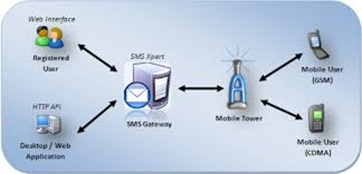
\includegraphics[width=0.6\textwidth]{gambar/sms_gateway}
\caption{\textit{Sistem SMS Gateway}}
\label{wsn}
\end{figure}
\newpage

Strukturisasi Pengaplikasian SMS Gateway Sebelum memulai lebih lanjut ada beberapa istilah yang perlu diketahui didalam SMS dan Koneksinya dengan Gateway perusahaan telekomunikasi (Telco) seperti kalau di Indonesia adalah Telkomsel, Indosat, dll.
\begin{figure}[ht!]
\centering
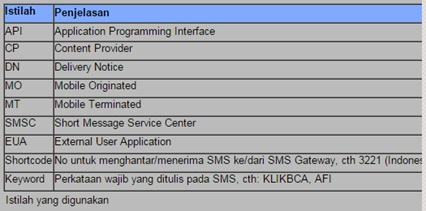
\includegraphics[width=0.6\textwidth]{gambar/Pengaplikasian_Gateway}
\caption{\textit{Struktur Pengaplikasian SMS Gateway}}
\label{wsn}
\end{figure}
\newpage

\section{Database}
Database adalah sistem penyimpanan beragam jenis data dalam sebuah entitas yang besar untuk diolah sedemikian rupa agar mudah dipergunakan lagi. Data yang disimpan bisa sangat variatif (angka, teks, gambar, suara, dan jenis data multi-media lainnya). Basis data merupakan kumpulan dari data yang saling berhubungan satu dengan yang lainnya, tersimpan di perangkat keras computer dan digunakan perangkat lunak untuk memanipulasinya. Database merupakan salah satu komponen yang penting dalam sistem informasi, karena merupakan basis dalam menyediakan informasi bagi para pemakai. (Sucipto, 2012: 137). Beberapa truktur data yang terkait dengan pembangunan database meliputi beberapa bagian yaitu diantaranya :

\subsection{MySQL}
MySQL merupakan sebuah basis data yang mengandung satu atau beberapa kolom. Tabel terdiri atas sejumlah baris dan setiap baris mengandung satu atau beberapa kolom. Didalam PHP telah menyediakan fungsi untuk koneksi ke basis data dengan sejumlah fungsi untuk pengaturan baik menghubungkan maupun memutuskan koneksi server database MySQL sebagai sarana untuk mengumpulkan informasi. (Yeni Kustiyahningsih, Devie Rosa Anamisa, 2010: 145-146).

MySQL adalah sistem manajemen basisdata relasi yang bersifat terbuka atau open source. Sistem manajemen basisdata ini adalah hasil pemikiran dari Michael “Monty” Widenius, David Axmark, dan Allan Larson pada tahun 1995. 

Tujuan awal ditulisnya program MySQL adalah untuk mengembangkan aplikasi web. MySQL menggunakan bahasa standar SQL (Structure Query Language) sebagai bahasa interaktif dalam mengelola data. 
Perintah SQL sering juga disebut Query. MySQL menawarkan berbagai keunggulan dibandingkan database server lain.

Berikut ini adalah beberapa keunggulan MySQL:
\begin{itemize}

\item[1.]	Mampumenanganijutaanuser dalamwaktu yang bersamaan.
\item[2.]	Mampumenampunglebihdari 50.000.000 record.
\item[3.]	Sangatcepatmengeksekusiperintah.
\item[4.]	Memilikiuser privilege system yang mudahdanefisien.
\end{itemize}

Kelemahan MySQL:
\begin{itemize}

\item[1.]	Untuk koneksi ke bahasa pemrograman visual seperti vb, delphi, dan foxpro, mysql kurang support, karena koneksi ini menyebabkan field yang dibaca harus sesuai dengan koneksi dari program visual tersebut, dan ini yang menyebabkan mysql jarang dipakai dalam program visual.
\item[2.]	Data yang ditangani belum begitu besar.
\end{itemize}

\subsection{Entity Relationship Diagram (ERD)}
Entity Relationship Diagram (ERD) merupakan bentuk dari hubungan antar file yang terjadi dalam program aplikasi. Pada model data relational hubungan antar file direlasikan dengan kunci relasi yang merupakan kunci utama dari masing-masing file. Dengan ERD dapat membuat sebuah relational condition atau hubungan antar elemen yang dapat diimplementasikan ke dalam bentuk tabel relasi.

Simbol-simbol yang digunakan dalam Entity Relationship Diagram dijelaskan pada tabel berikut ini :
\begin{figure}[ht!]
\centering
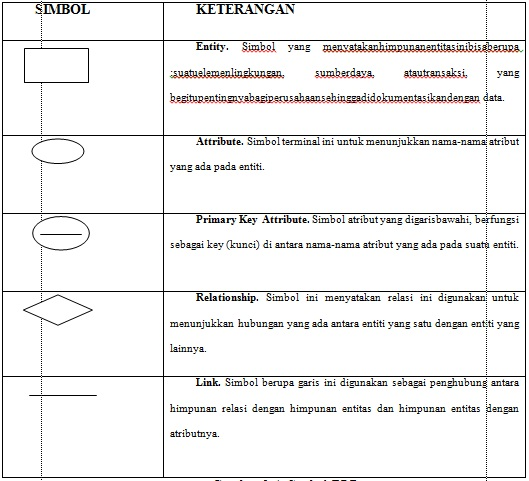
\includegraphics[width=0.8\textwidth]{gambar/Simbol-ERD}
\caption{\textit{Simbol ERD}}
\label{wsn}
\end{figure}
\newpage

Dalam ERD hubungan (relasi) dapat terdiri dari sejumlah enntitas yang disebut dengan derajat relasi. Derajat relasi maksimum disebut dengan kardinalitas sedangkan derajat minimum disebut dengan modalitas. Jadi kardinalitas relasi menunjukkan jumlah entitas yang dapat berelasi
	
Dengan entitas pada himpunan entitas lain. Kardinalitas relasi yang terjadi diantara dua himpunan entitas (misalnya A dan B) dapat berupa :
\begin{itemize}

\item[1.]	Satu ke satu (One to One/ 1-1)

Setiap entitas pada himpunan entitas A dapat berelasi dengan paling banyak satu entitas pada himpunan B, demikian juga sebaliknya.
\item[2.]	Satu ke banyak (One to Maty/ 1-N)

Setiap entitas pada himpunan entitas A dapat berelasi dengan banyak entitas pada himpunan entitas B, tetapi tidak sebaliknya.
\item[3.]	Banyak ke banyak (Many to Many/ N-N)

Setiap entitas pada himpunan entitas A dapat berelasi dengan banyak entitas pada hhimpunan entitas B, demikian juga sebaliknya.

(Sumber : http://www.ilmukomputer.com/IX ERD.pdf)
\end{itemize}

\subsection{Conceptual Data Model (CDM)}
Merupakan sebuah model pendekatan secara konsep sebelum dikonversi menjadi model data fisik yang telah berkaitan dengan tujuan basis data tertentu. Skema konseptual atau model data konseptual adalah sebuah peta konsep dan hubungan mereka yang digunakan pada sebuah database. Pada perancangan model konseptual akan menunjukkan entity dan relasinya berdasarkan proses yang diinginkan ole organisasi. Pendekatan yang dilakukan pada perancangan model konseptual adalah dengan menggunakan model data relational.

Manfaat penggunaan CDM dalam perancangan database :
\begin{itemize}

\item[1.] Memberikan gambaran yang lengkap dari struktur basis data yaitu arti, hubungan, dan batasan-batasan.
\item[2.] Alat komnikasi antar pemakai basis data, designer, dan analisis.
\end{itemize}

Jenis-jenis obyek dalam CDM :
\begin{itemize}

\item[1.]	Entity
\item[2.]	Relationship
\item[3.]	Inheritance
\item[4.]	Association
\end{itemize}

Berikut contoh CDM :
\begin{figure}[ht!]
\centering
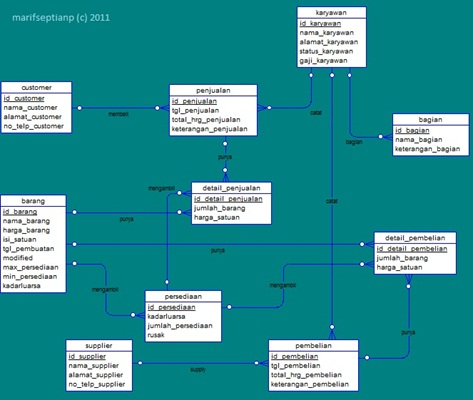
\includegraphics[width=0.8\textwidth]{gambar/CDM}
\caption{\textit{Contoh CDM}}
\label{wsn}
\end{figure}
\newpage

\subsection{Physical Data Model (PDM)}
Merupakan model yang menggunakan sejumlah tabel untuk menggambarkan data serta hubungan antara data-data tersebut. Setiap tabel mempunyai sejumlah kolom dimana setiap kolom memiliki nama yang unik.

Jenis-jenis objek dalam PDM :
\begin{itemize}

\item[1.] Tabel
\item[2.] View
\item[3.] Reference
\end{itemize}
Menurut ANSI, arsitektur basis data terbagi atas tiga level, yaitu :
\begin{itemize}

\item[1.] Internal / Physical Level, (yang dapat diimpresentasikan dengan PDM) berhubungan dengan bagaimana  data disimpan secara fisik (Physical storage).
\item[2.] External / View Level, berhubungan dengan bagaimana data di representasikan dari sisi setiap user.
\item[3.] Conceptual / Logical Level, (yang dapat direpresentasikan dengan CDM) yang menghubungkan antara internal dan external level.
\end{itemize}

Berikut contoh PDM :
\begin{figure}[ht!]
\centering
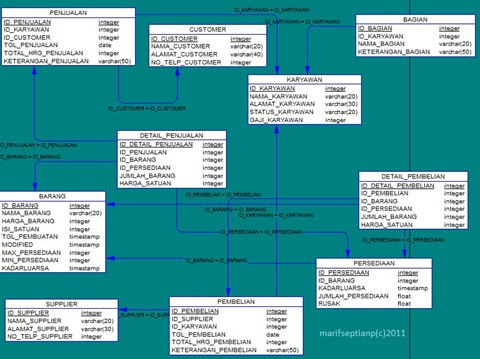
\includegraphics[width=0.8\textwidth]{gambar/PDM}
\caption{\textit{Contoh PDM}}
\label{wsn}
\end{figure}
\newpage

\section{Tinjauan Umum Tools Perancangan Sistem}
\subsection{System Flowchart}
Menurut Raymond Jr McLeod menyatakan bahwa System Flowchart merupakan bagan yang mennjukkan arus pekerjaan secara keseluruhan dari sistem. Bagan ini menjelaskan tahapan-tahapan dari prosedur-prosedur yang ada di dalam sistem. Flowchart menunjukkan apa yang dikerjakan di sistem. 
\newpage
Simbol-simbol yang digunakan dalam system flowchart adalah sebagai berikut :
\begin{figure}[ht!]
\centering
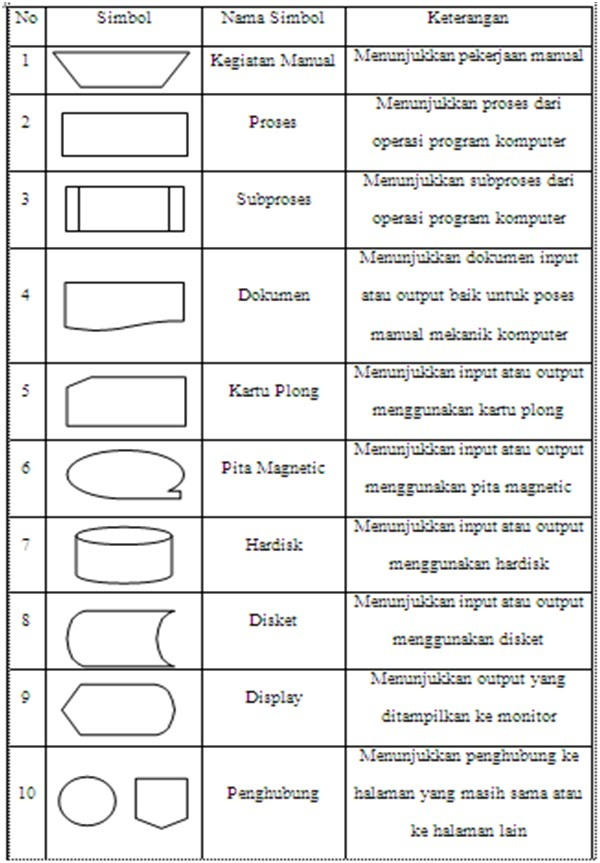
\includegraphics[width=0.8\textwidth]{gambar/Simbol-Flowchart}
\caption{\textit{Simbol Flowchart}}
\label{wsn}
\end{figure}

\subsection{Data Flow Diagram (DFD)}
Data Flow Diagram (DFD) adalah diagram yang menggunakan notasi-notasi untuk menggambarkan arus dari sistem. DFD sering digunakan untuk menggambarkan suatu sistem yang telah ada atau system baru yang akan dikembangkan secara logika tanpa mempertimbangkan lingkungan fisik dimana data tersebut mengalir (misalnya lewat telepon, surat, dan sebagainya) atau lingkungan fisik dimana data tersebut akan disimpan (misalnya file kartu, hard disk, tape, diskette, dan lain sebgainya).

Simbol-simbol yang digunakan di DFD mewakili maksud tertentu, yaitu:
\begin{itemize}

\item[1.]	External entity (kesatuan luar) atau boundary (batas sistem)
Setiap system pasti memiliki batas sistem (boundary) yang memisahkan suatu system dengan lingkungan luarnya. Kesatuan luar (external entity) merupakan kesatuan di lingkungan luar sistem yang dapat berupa orang, organisasi atau system lainnya yang berada di lingkungan luarnya yang akan memberikan input atau menerima output dari sistem.
Gambar notasi kesatuan luar DFD:

\begin{figure}[ht!]
\centering
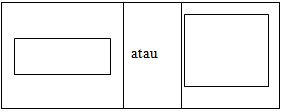
\includegraphics[width=0.6\textwidth]{gambar/Eksternal}
\label{wsn}
\end{figure}

\item[2.]	Data flow (arus data)
Arus data di DFD diberi symbol panah. Arus data ini mengalir diantara proses, simpanan data dan kesatuan luar.

Gambar symbol arus data pada DFD:

\begin{figure}[ht!]
\centering
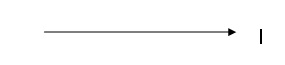
\includegraphics[width=0.6\textwidth]{gambar/Arus-Data}
\label{wsn}
\end{figure}

\item[3.]	Process (proses)
Suatu proses adalah kegiatan atau kerja yang dilakukan oleh orang, mesin atau computer dari hasil suatu arus data yang masuk kedalam proses untuk dihasilkan arus data yang akan keluar dari proses.

\newpage
Gambar simbol proses pada DFD:
\begin{figure}[ht!]
\centering
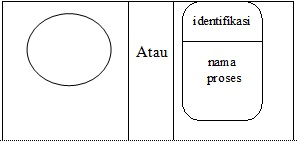
\includegraphics[width=0.4\textwidth]{gambar/Proses}
\label{wsn}
\end{figure}

\item[4.]	Data store (simpanan data)
Simpanan data (data store) merupakan simpanan dari data yang dapat berupa suatu file atau database di komputer, suatu arsip atau catatan manual, dan lain sebagainya. 
Simpanan data di DFD dapat disimbolkan sebagai berikut:
\begin{figure}[ht!]
\centering
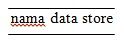
\includegraphics[width=0.4\textwidth]{gambar/Simpanan}
\label{wsn}
\end{figure}

\end{itemize}

%-------------------------------------------------------------------------------
\chapter{METODOLOGI PENELITIAN}

\section{Metode Penelitian}
Metode penelitian yang digunakan dalam proses penyelesain aplikasi distribusi informasi berbasis SMS Gateway  terdiri dari berbagai tahapan. Tahapan-tahapan yang dimaksud dijelaskan pada diagram sebagai berikut :

\begin{figure}[ht!]
\centering
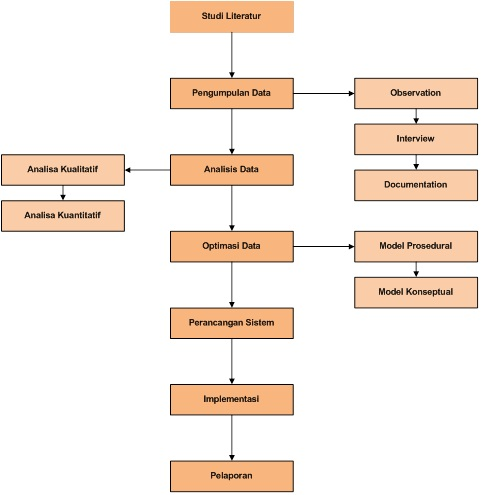
\includegraphics[width=1\textwidth]{gambar/BaganMetode}
\caption{Bagan Metode Penelitian}
\label{wsn}
\end{figure}
\newpage

\subsection{Studi Literatur}
Studi Literatur dilakukan untuk mengetahui dan mengkaji secara teoritis, metode yang dipakai untuk memecahkan masalah yaitu dengan cara mencari data-data yang berhubungan dengan sistem pemberian informasi.

\subsection{Pengumpulan Data}
Pada tahap ini dilakukan pengumpulan data yang diperlukan dengan maksud untuk memperoleh data yang relevan, akurat dan sesuai dengan tujuan penelitian. Pada penelitian ini metode pengumpulan data dilakukan dengan 3 cara yaitu :
\begin{itemize}

\item[1.]	Observation, yaitu dalam hal ini penulis melakukan pengamatan secara langsung kelapangan untuk mencari permasalahan yang dihadapi oleh sistem penyampaian informasi di Organisasi Himpunan Mahasiswa Islam.
\item[2.]	Interview, yaitu mengadakan wawancara dengan beberapa koresponden yang berada di lapangan yang dianggap tepat dijadikan sebagai nara sumber atas permasalahan yang terjadi.
\item[3.]	Documentation, yaitu melakukan survei data dengan melihat data–data berupa document atau data tertulis yang sudah ada dalam data sebelumnya seperti ; data agenda kegiatan yag telah dilaksanakan.
\end{itemize}

\subsection{Analisis Data}
Proses analisis data itu dimulai dari menelaah data secara keseluruhan yang telah tersedia dari berbagai macam sumber, baik itu pengamatan, wawancara, catatan lapangan dan yang lainnya. Analisa data dapat dibedakan menjadi dua yaitu analisa kualitatif dan analisa kuantitatif.
\begin{itemize}

\item[1.]	Analisa Kualitatif

yaitu analisa mengambarkan dengan kata-kata atau kalimat yang dipisah-pisahkan menurut kategori untuk memperoleh kesempatan.


\item[2.]	Analisa Kuantitatif

merupakan analisa yang berwujud angka-angka hasil perhitungan atau pengukuran yang diproses untuk mendapat data unit.
Dalam penulisan tugas akhir ini teknik analisis data yang penulis gunakan adalah analisis kualitatif.
\end{itemize}

\subsection{Optimasi Data}
Optimasi data pada penelitian ini dapat berupa model prosedural, model konseptual. 
\begin{itemize}

\item[1.]	Model prosedural adalah model yang bersifat deskriptif, yaitu menggariskan langkah – langkah yang harus diikuti untuk menghasilkan sistem yang baik. 
\item[2.]	Model konseptual adalah model yang bersifat analitis yang memberikan komponen – komponen sistem yang akan dikembangkan serta keterkaitan antara sistem yang akan digunakan pada sistem HMI. Agar pada sistem akhir yang diperoleh dapat menghasilkan sistem yang baik dan akurat.
\end{itemize}

\subsection{Perancangan Sistem}
Pada tahap perancangan sistem dimaksudkan agar sistem yang dibuat sesuai dengan kebutuhan penggunaan bagi admin atau para anggota HMI dalam penyampaian informasi dan dapat berjalan dengan baik, pada perancangan sistem ini penulis menggunakan cara sebagai berikut :
\begin{itemize}

\item[1.]	Perancangan Sistem Informasi

Merancang suatu sistem informasi dengan tools perancangan berupa flowchart, DFD, dan ERD untuk menggambarkan proses distribusi informasi.

\item[2.]	Pembangunan Database

Pembuatan struktur database diambil dari rancangan ERD, CDM, PDM sebelumnya sehingga menghasilkan suau database yang nantinya akan dibuat.
\end{itemize}

\subsection{Implementasi}
Dalam implementasi sistem dilakukan untuk menerapkan perangkat lunak yang dihasilkan ke permasalahan yang dihadapi pengguna sebagai sebuah solusi agar aplikasi ini bisa berjalan lebih sempurna. Tahap implementasi sistem terdiri dari beberapa langkah sebagai berikut :
\begin{itemize}

\item[1.]	Menerapkan Rencana Implementasi

Rencana implementasi dimaksudkan untuk mengatur waktu yang dibutuhkan selama melakukan tahap implementasi dan biaya yang akan diperlukan selama itu.

\item[2.]	Melakukan Kegiatan Implementasi

Kegiatan yang dilakukan dalam tahap implementasi ini adalah sebagai berikut :
\end{itemize}

\begin{itemize}

\item[1.]	Pemrograman (Coding Program)

Adalah suatu kegiatan mneulis kode program yang akan dilakukan pada project yang dikerjakan dan akan dieksekusi oleh komputer. Kode program yang ditulis harus sesuai dengan dokumentasi data yang telah didapatkan oleh analisis sistem dari suau desain sistem yang secara rinci. Hasil program yang sesuai dengan sistem yang ada, akan menghasilkan suatu program yang dibutuhkan oleh pemakai sistem.
\item[2.]	Uji Coba Program

Adalah suatu kegiatan untuk mengetahui kesalahan atau kekurangan yang mungkin akan terjadi dalam pembuatan program tersebut.
\end{itemize}

\subsection{Pelaporan}
Proses dan hasil penelitian yang telah diperoleh dituangkan dalam bentuk laporan Tugas Akhir.

\section{Desain Sistem}
Merupakan suatu tahap pengembangan sistem yang mendefinisikan dari kebutuhan fungsional, persiapan untuk rancang bangun, menggambarkan bagaimana sistem yang akan dibentuk. Penggambaran rancangan sistem distribusi informasi berbasis sms gateway yang akan dibuat dapat digambarkan dalam bentuk flowchart sistem. Flowchart sistem yang akan dibuat berisikan tentang persiapan kebutuhan untuk membangun sistem tersebut.

\begin{figure}[ht!]
\centering
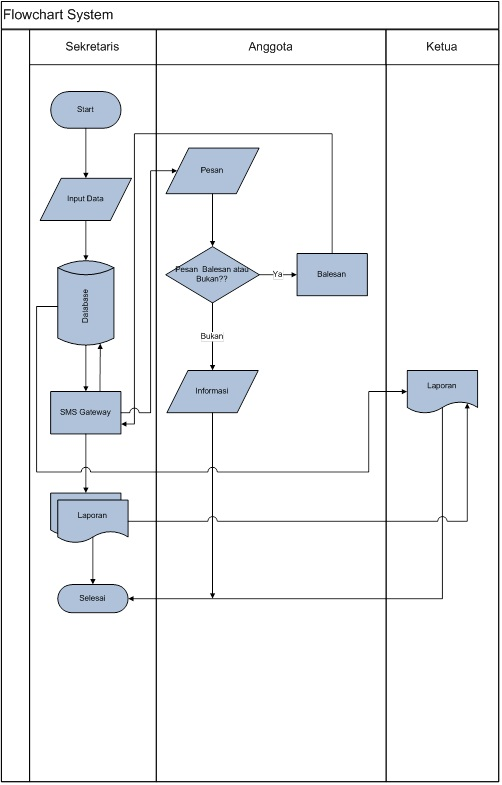
\includegraphics[width=0.8\textwidth]{gambar/Flowchart_sistem}
\caption{\textit{Flowchart Sistem}}
\label{wsn}
\end{figure}
\newpage

Keterangan:
\begin{itemize}

\item[1.]	Sekretaris, mempunyai peran tentang proses pengolahan data dimana proses yang dilakukan terkait dengan penginputan data, seperti misalnya data-data para anggota, struktur organisasi, dan agenda kegiatan yang telah terstruktur.
\item[2.]	Data yang telah diinputkan akan ditampung dan disimpan  kedalam suatu database.
\item[3.]	Selanjutnya, dari proses penyimpanan database komputer akan mengirimkan pesan sesuai dengan agenda kegiatan yang sudah dijadwalkan sebagai informasi kepada para anggota dengan sistem sms gateway.
\item[4.]	Jika pesan tersebut berupa suatu  informasi yang menginginkan balasan, maka anggota akan memberikan suatu balasan sebagai hasil poling dari informasi tersebut.
\item[5.]	Jika pesan hanya sebagai informasi saja maka pesan selesai dan ditrima.
\item[6.]	Pada proses balasan pesan tersebut, poling balasan akan ditampung dan disimpan dalam database.
\item[7.]	Setelah poling balasan ditampung dan disimpan dalam database, sistem sms gateway akan memberikan suatu laporan.
\item[8.]	Laporan tersebut berkaitan dengan arsip dari data kegiatan yang telah diselenggarakan maupun yang akan dilaksanakan berupa suatu hardcopy.
\end{itemize}


\section{Alat Bantu}
Untuk kelancaran dalam penelitian ini, berikut penjelasan mengenai alat bantu yang penulis gunakan, yaitu :

\subsection{Perangkat Keras (Hardware) }

yang digunakan dalam pembuatan perancangan sistem ini adalah satu unit Laptop dengan spesifikasi sebagai berikut :
\begin{itemize}

\item[a.]	Processor	: Intel ® Core ® CPU
 P6200 @ 2.40 Ghz
\item[b.]	Memori	: 2 GB DDR3 Memory
\item[c.]	Hardisk	: 32 GB HDD
\end{itemize}

\subsection{Perangkat Lunak}
untuk mempermudah software yang digunakan dalam penyusunan Aplikasi ini antara lain :
\begin{itemize}

\item[a.]	Microsoft Office Word 2010
\item[b.]	Microsoft Office Visio 2007
\item[c.]	Sybase Power Designer 15.0
\item[d.]	NetBeans IDE 7.0.1
\end{itemize}


\section{Pengujian}
Proses pengujian dapat dilakukan setelah aplikasi yang dibuat telah selesai. Tujuan pengujian adalah untuk memastikan aplikasi yang dibuat benar-benar bisa digunakan atau masih mengalami kesalahan. Proses pengujian aplikasi tersebut dimulai dari penginputan data-data yang ada pada agenda kegiatan dan menyimpannya kedalam database, setelah data tersimpan, maka sistem sms gateway akan melakukan prosess broadcasting pesan kepada para anggota. Pesan tersebut memiliki dua tipe yaitu berupa pesan balasan informasi dan pesan hanya sebagai informasi saja.

\section{Rencana Jadwal Penulisan/Kegiatan}
Dalam melaksanakan tahapan penilitian agar penelitian tersebut dapat diselesaikan sesuai dengan waktu yang direncanakan maka peneliti membuat matrik berupa tahapan jadwal penelitian sebagai berikut:
\begin{table}[ht!]
\centering
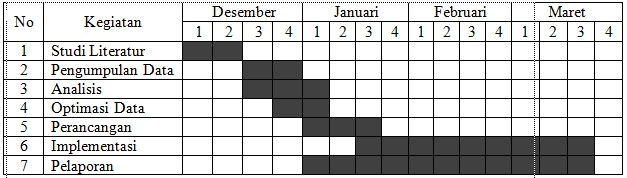
\includegraphics[width=1\textwidth]{gambar/Jadwal-Ayu}
\caption{\textit{\textit{Jadwal Kegiatan}}}
\label{wsn}
\end{table}
\newpage

\end{document}